\documentclass{cpeauth}

\usepackage[numbers, sort, compress]{natbib}
\usepackage{graphics}
\usepackage{graphicx}
\usepackage{epstopdf}
\usepackage{color}
\usepackage{hyperref}
\usepackage{pdfsync}
\usepackage{mdwlist}

\usepackage{colortbl}

\usepackage{wrapfig}
\usepackage{floatrow}
\newfloatcommand{capbtabbox}{table}[][\FBwidth]
\usepackage{blindtext}


\begin{document}

%\conferenceinfo{ccpe,} {}
%\CopyrightYear{2011}
%\crdata{}
%\clubpenalty=10000
%\widowpenalty = 10000


\def\cop{Copyright \copyright\ 2000 John Wiley \&\ Sons, Ltd.}
%\CPE{1}{6}{00}{00}{2000} %for times fonts
\CPE{1}{7}{00}{00}{2000}



\newif\ifdraft
\drafttrue

\ifdraft
% \newcommand{\reviewer}[1]{ {\textcolor{blue}    { ***Reviewer:     #1 }}}
 \newcommand{\jkimnote}[1]{{\textcolor{green}   { ***Joohyun:   #1 }}}
% \newcommand{\jhanote}[1]{  {\textcolor{red}     { ***SJ: #1 }}}
 \newcommand{\jhanote}[1]{}
 \newcommand{\jhanew}[1]{{\textcolor{red}     { ***SJ: #1 }}}
  \newcommand{\smnote}[1]{  {\textcolor{red}     { ***Sharath: #1 }}}
  \newcommand{\msnote}[1]{  {\textcolor{blue}     { ***Mark: #1 }}}

 \newcommand{\todo}[1]{  {\textcolor{red}     { ***TODO: #1 }}}
 \newcommand{\fix}[1]{  {\textcolor{red}     { ***FIX: #1 }}}
 \newcommand{\reviewer}[1]{}
\else
 \newcommand{\reviewer}[1]{}
 \newcommand{\jkimnote}[1]{}
 \newcommand{\smnote}[1]{}
 \newcommand{\jhanote}[1]{}
 \newcommand{\jhanew}[1]{}
\newcommand{\todo}[1]{  {\textcolor{red}     { ***TODO: #1 }}}
 \newcommand{\fix}[1]{}                                                                                     
\fi


\title{Advancing Next-Generation Sequencing Data Analytics with Scalable Distributed Infrastructures}


\author{
Joohyun Kim\ensuremath{^1} \comma, %\footnotemark[2], 
Sharath Maddineni\ensuremath{^1},
%Mark Santcroos\ensuremath{^1,^2},
Shantenu Jha\corrauth\ensuremath{^2,^1} %\comma, %\footnotemark[3],
}

\longaddress{\ensuremath{^1}Center for Computation and Technology, Louisiana State University, LA, USA\\ 
\ensuremath{^2}Rutgers University, Piscataway, NJ 08854, USA}

\date{}

\received{}
\revised{}
\noaccepted{}

\begin{abstract} 
  Next Generation DNA Sequencing produce significantly larger amounts
  of data compared to early sequencing methods based on Sanger
  technology.  Along with challenges arising from unprecedented
  volumes of data, a research is increasingly dealing with the
  requirement of effectively analyzing the data, in particular with
  the emergence of popular NGS-based genome-wide protocols such as
  ChIP-Seq and RNA-Seq.  In this work, we use BFAST, a mapping
  program, as a representative standalone tool used for NGS data
  analysis, and a ChIP-Seq pipeline that is composed of two main
  steps, i.e. a mapping and a peak calling task with small other
  tasks, as a representative pipeline-based approach.  With BFAST, we
  analyzed computational requirements using two model genomes -- human
  genome and a microbe ({\it Burkerholderia Glumae}), that represent
  an eukaryotic and a prokaryotic system.  For the ChIP-Seq pipeline,
  experimental data probing genome-wide chromatin structure of mouse
  was used.  The computational complexity of genome-wide mapping using
  BFAST, amongst other factors depends upon the size of a reference
  genome, the data size of short reads. We analyze the performance
  characteristics of BFAST and understand its dependency on different
  input parameters. Characterizing the performance suggests that
  genome-wide mapping benefits from both scaling-up (increased
  fine-grained parallelism) and scaling-out (task-level parallelism --
  local and distributed).  For certain problem instances, scaling-out
  can be a more efficient approach than scaling-up.  Importantly, with
  our investigation on the pipeline for ChiP-Seq, we discuss that the
  importance of dynamical execution of tasks comprising a pipeline for
  NGS data, and that the support of scalability, flexibility, and
  extensibility should be considered as an important aspect, besides
  much focused algorithmic or implementation strategies, for
  leveraging existing or new-generation of pipeline developments for
  NGS data.  We then describe the design and development of a
  runtime-environment, Dynamic Application Runtime Environment (DARE),
  that supports both the scale-up and scale-out of BFAST on production
  grid and cloud environments, and the effective ChIP-seq Pipeline on
  scalable distributed infrastructures.


\end{abstract}

%\category{D.1.3}{Software}{Concurrent Programming}{ Distributed
%  programming/parallel programming} \category{J.3}{Computer
%  Applications}{Bioinformatics, Mapping}
%
%
%% A category with the (minimum) three required fields
%%\category{H.4}{Information Systems Applications}{Miscellaneous} %Acategory including the fourth, optional field follows...
%%\category{D.2.8}{Software Engineering}{Metrics}[complexity measures,performance measures]
%
%\section*{General Terms}{Performance,Measurement,Theory}
%
% \keywords{Genome
%  Sequence Alignment, BFAST, Human Genome, Burkerholderia Glumae,
%  Runtime Environment, Distributed Computing, Simple API for Grid
%  Applications (SAGA), Pilot-Job abstraction}
%
%%\keywords{ACM proceedings, \LaTeX, text tagging} % NOT required for Proceedings 
%%\keywords{RNA conformation energy landscape, Runtime Environment, SAM-I riboswitch,
%% S gene of Bovine Corona Viral Genome} % NOT required for Proceedings

 \keywords{Next-Generation Sequencing Data Analytics, Science Gateway, BFAST, ChIP-Seq, Human Genome, Burkerholderia Glumae, Runtime Environment, Distributed Computing, Simple API for Grid Applications (SAGA), Pilot-Job abstraction}


\section{INTRODUCTION} 

\jhanote{- How other infrastructure + tools that have been used to support NGS on DCI (including comparision with DIANE as a solution)
- Type III  -- workflows + dyn Execution for NGS}


%\reviewer{R-7 : Kim and colleagues explore fine and coarse-grained parallelism of one next-gen sequencer in their DARE framework.  Rather than take a bioinformatics/cloud tack like the Salzberg group at Maryland (and others), they propose their custom framework as a gateway for next-gen sequencing analysis.  
%Philosophically, this problem is no different from the BLAST problem that was published in a few papers last year in this workshop.  It is also unclear to me the distinction between DARE, SAGA-BigJob, and ADAMS previously reported by these authors in this workshop, mostly because they are flavors of SAGA-BigJobs and the limitations of a "distributed programming environment" discussed in the ADAMS paper is also applicable here.  Mapreduce and other abstractions are used in this community -- and I am not saying always used well -- because they are in some sense easier to program.  My opinion is that the advances in workflows must accompany improvements in infrastructure, but I recognize where they are coming from.  I agree that the nature and amount of parallelism is different between DARE and ADAMS and this is an emerging problem of interest to the life sciences community.  My suggestions for the authors prior to publication are to adequately address the scaling contribution more than the application engineering aspect herein.  Detailed comments follow that outline this logic.  A consequence of knowing this area well is often a longer (and in a sense harsher review) but I find this work interesting just needs more information on the HPC side to fully support their claims in a self contained manuscript.}
%
%\reviewer{R-7 : I guess BFAST was chosen because it is multithreaded and fits into the DARE framework; however,it is one of the least used short read aligners mostly because it is based on a suffix array that is voracious either in memory or disk.  These issues are mentioned in the manuscript indirectly but no thought is given how to scale out a job that would require 200GB of local space.  BWA and the Bowtie, both based on the Burrow-Wheeler transform, are more practical tools to look at for run time needs mostly because they are the more popular (216 and 382 Google scholar citations, respectively, vs. 26). Bowtie, cited here,also has been ported to a cloud environment as mentioned by these authors. The authors should strongly consider comparison to other frameworks (esp. bowtie) for a fair comparison of the practical benefit of their approach.}\jkimnote{we will put some sentences why Bfast is chosen other than other popular ones such as BWA or Bowtie that use BWT and requiring less memory-basically BFAST aims the higher sensitivity in spite of larger memory requirement and more computing time, which might be the case whose effectiveness is further enhanced by scale-out approach}
%
%\reviewer{R-7 : Relatedly, the paper is very hard to evaluate with respect to its impact on life sciences. To be fair, the authors care more from the HPC/infrastructure side but ultimately the users of this software/gateway will come from outside of the HPC community.  The number one concern for scalability is the size of the index files and the state of the parallel I/O system, but these are not given in Tables 5-7.  It would have been very helpful to connect the examples in Table 3 to the results of the paper.  I will agree with the authors that the size of the query is important and is a key variable in Figures 5-7 but it discounts the practical concerns of parallelizing a tool like BFAST, which constructs a suffix array.  Please clarify what data is which for these tables so biologists can better evaluate the usefulness of the system.
%}
%
%\reviewer{R-7 : I would have liked to see ideally a complete workflow on the grid or cloud or scaling (and ideally both) not a statement related to overhead that, although true, does not support scaling as well as empirical results.
%}
%
%\reviewer{R-2 :First, the summary of existing efforts on cloud computing of NGS read mapping is not comprehensive. For example, the work by Salzberg and colleagues "Searching for SNPs with cloud computing" Genome Biology 2009 was not mentioned. }\jkimnote{this reference is already referred as ref. 20}
%
%\reviewer{R-3 : Aside from small textual errors (the authors should define the term CAL before using it, and some explanation of machine names such as Eric and Painter would be useful outside of tables and captions before we encounter them in text) I see no faults with the paper, but it amounts to little more than benchmarking with some explanations of the results.}\jkimnote{The definition of CAL is already in the figure 1 and the caption, but we should mention it again in the text. Sharath, can you find the description for Eric and Painter from the previous ECMLS10 or CCPE paper and put it in the figure caption?} 


High-throughput genome sequencing techniques provided by Next
Generation Sequencing (NGS) platforms are changing biological sciences
and biomedical research
dramatically\cite{mardis2008-tig,mardis2008-arghg}. These techniques
have led to a broadening of sequencing capabilities and access to
comprehensive genome-wide information at increasingly lower costs
compared to previous sequencing techniques (such as those based on
Sanger sequencing)
\cite{metzker2010,mardis2008-tig,mardis2008-arghg,gilad2009,mortazavi2008,sorek2010}.
Thanks to advances in deep sequencing protocols such as ChIP-seq
(chromatin immunoprecipitation-seq) and RNA-seq, high-throughput
sequencing techniques have become essential methodologies in studies
of cell development and
differentiation\cite{wang2009-natrevgen,pepke2009,gilad2009,mortazavi2008,sorek2010}.
Indeed, the resulting influx of biological information about the
genome-wide organization and the interaction map of target genes and
pathways reveal underlying mechanisms of gene expression and
regulation in living cells. This has the potential to lead to remedies
for various diseases such as cancer, infectious diseases, and
dysfunctional diseases caused genetically or by
aging\cite{amaral2008,encode2007,baek2008,costa2009}.


High-throughput techniques enjoy extremely high coverage of target
genome regions; current "deep sequencing"
technologies adopted by NGS platforms such as Illumina GA II
and Applied Biosystems SOLiD are limited to generating only short
sequence reads, generally less than 100 hundred
nucleotides\cite{metzker2010}.

Consequently, it has become a computational challenge to map these
high volume short reads onto a reference genome or de novo assembly
that are needed as the first step for any genome-wide
studies\cite{alex2009,trapnell2009,scheibye-alsing2009,pop2002,hernandez2008,farrer2008}.
It is expected that data-sets of interest will increase by several
orders of magnitude as the number of genomes that need to be sequenced
together increases exponentially.  This is a result of comparative
genomics as well as genome-wide variation studies that require a
statistical number of genomes for one single species as shown in the
recent 1000 genome project and human genome
studies\cite{1000genome,mardis2008-tig,gilad2009,alex2009,kim2011}.

%challenge immediately mapping process on to a reference genome or 
% Consequently, these high volume short reads challenge immediately
% mapping process on to a reference genome or de novo assembly that are
% needed as the first step for any genome-wide
% studies\cite{alex2009,trapnell2009,scheibye-alsing2009,pop2002,hernandez2008,farrer2008}.

To address these challenges, there have been algorithmic advances and
several tools implementing these advances are becoming available
\cite{trapnell2009,bfast2009,scheibye-alsing2009,pepke2009,samtools}.
Whereas such algorithmic advances and introduction of new tools have
been consistently led by the computational biology community, the
development of a well-architected integrated infrastructure -- the
software \& services, data management capabilities and user interfaces
has received less attention.  As we will demonstrate, NGS analysis is
not a simple compute or data-intensive application, but an interesting
mix of high-end and high-throughput computing with data-intensive
requirements.  We ask the fundamental question: what is the
appropriate architecture of the infrastructure to address the existing
computational requirements of NGS analysis, data-set volumes -- now
and extrapolating into the future?  The need for an appropriate
scalable and flexible architecture for the infrastructure, becomes
prevalent because the computational complexity of the specific problem
instance is often influenced by the biological characteristics of 
target genome(s) and the volume of relevant genomics data.

%\jhanote{not sure what to do with the following paragraph} One
%important caveat is that as advances of genome sequencing technologies
%evolve further in the future with innovations, for example, such as a
%single molecule sequencing technology and ever-growing genome data,
%any computational algorithms or implementations with a bioinformatic
%tool are subject to change to respond such progresses or will become
%less useful if the tool do not meet new conditions.

Our approach is to primarily focus on the mapping process of short
reads from NGS platforms against a reference genome.  The mapping is
carried out with the tool, BFAST\cite{bfast2009, bfast2009b} which was
chosen specifically considering its capability to support parallel and
multi-threading execution.
It is noted that BFAST was developed to achieve high sensitivity and accuracy, where as BWA and Bowtie employed efficient memory usage and require lower data volume\cite{bfast2009}.
 The choice of this tool is appropriate for our purposes, as this % Indeed, our investigation
% with this bioinformatic program would
is a representative situation for a bioinformatics tool enhanced
considerably for genome-wide analysis with scalable infrastructure.

% \reviewer{R-7 : "an existing framework -- which enables the seamless
%   utilization of heterogenous resources" and When I think of seamless
%   utilization of heterogeneous resources I think of swift, work
%   queue/makeflow, and other lightweight "ad hoc" cloud systems.  The
%   contribution here is that compiling BFAST in the DARE framework
%   allows using different resources, but not at the same time?  It is
%   unclear without reading the previous work why this is an improvement
%   on something like swift or other workflow-enabling lightweight
%   frameworks.  } 

As a use case, we analyze the computational complexity of
BFAST\cite{bfast2009, bfast2009b} and the determinants of its
performance for two exemplary genomes, human genome and a microbial
genome {\it Burkerholderia Glumae}\cite{kim2011}.  Having understood
the computational requirements, and the importance of both scaling-up
and scaling-out, we present the initial design objectives and a
prototype of an infrastructure that seamlessly uses High-Performance
Computing (HPC) grids and Cloud environment for genome-wide analysis.
Our infrastructure builds upon existing capabilities of the Dynamic
Application Runtime Environment (DARE) framework\cite{tg11} -- which
enables the seamless utilization of heterogeneous distributed
computing resources\cite{saga-iccs09,saga-royalsoc,saga-ccgrid10}.
DARE provides an existing efficient framework upon which to build a
scalable infrastructure to support a wide range of abstractions and
execution requirements for the analytics required for NGS
data. \reviewer{R-7 : ""an existing efficient framework upon which to
  build a scalable infrastructure to support a wide range of
  abstractions and execution environments.""  When I think efficient,
  I usually think of the HPC concept of speedup / number of processors
  or a more loosely defined programability argument.  None of the
  traditional measures are present in this paper.  For example, in
  Table 6 the framework appears to scale to at least 80 cores but I
  have at least three concerns with these data: 1.)  how long did the
  job take on a serial system, and therefore what is the speedup on
  the grid/cloud?  2.)  Were the authors able to process a complete
  run of either the human or Burkerholderia? This is unclear from the
  abstract examples. 4.) Does the grid/cloud version provide speedup
  over a plain threaded version of BFAST on similar hardware?  5.)  No
  ability to measure how scalable the software is as there are only
  two data points on an HPC grid (LONI) that I assume had a shared
  file system?  The same number of cores were used in Table 7. }
\smnote{ 1) Lets say we have "n" read files and with DARE it takes
  around time "t" time for matching step if we run it serially it
  would take n*t time. It probably exceeds wall time limit. Therefore
  speed up in match step depends how many number of read files we
  generate and process concurrently.  2) Yes we were able to process
  the complete run with entire Human Genome on QB and Ranger
  separately. (**I am currently working this to utilizing QB and
  Ranger together.)  4) it should clearly provide the advantage with
  multiple resources. If we want to use the cloud resources from India
  to complete Human Genome run it is not practically possible because
  of the current limited disk size access provided by the FG
  Eucalyptus resources. Because whole human genome index files are of
  size 129 GB for Bfast matching step as opposed to HG 18 Chromosome
  21 with size of 2 GB index files. On the other hand it also requires
  the temporary files disk space.  Thus it is important to utilize
  large capacity resources like QB and Ranger divide the work load
  across machines.} \jhanew{Sharath, JK: Please remove comments that
  have been fixed. Has this been addressed?}

Our infrastructure has distinctive characteristics, compared to other
related approaches\cite{taylor2010,cloudburst, cloudblast,
  langmead2009,langmead2010,gatk,halligan2009,luyf-2010}, many of
which have been developed in the Cloud environment.  First of all,
most other approaches lack interoperability between different
distributed computing environments.  This is partly because the
application layer is tightly coupled to the runtime environment layer.
Secondly, other approaches support a single or closely related few
applications.  The main design strategy of the DARE framework is to
separate the application logic from a target tool(s), consequently
resulting in easy-to-develop cycles for improvement, changes, and
deployment of new tools.  % On the other hand, it is also true that
Some tools such as CloudBurst\cite{cloudburst},
CloudBlast\cite{cloudblast}, Crossbow\cite{langmead2009}, and
GATK\cite{gatk} have advantages that are specifically confined to
Cloud environments, as well as permit ease of utilization of effective
programming models such as MapReduce or other software frameworks,
whereas others\cite{luyf-2010} focus on the HPC grid environment.  Indeed, the DARE framework propose an interesting mean to support dynamic applications.

This paper is organized as follows.  We introduce BFAST and a ChIP-Seq pipeline with
their characteristic features with respect to computational and data
requirements.  In the following section, we examine
details on execution of BFAST, as a demonstrative mapping tool representing a simple category of dynamic application, using a local resource and then two distributed environments, a HPC grid and a cloud and on execution of the ChIP-Seq pipeline, as a more complex example for dynamic applications. Finally, we conclude with the summary of this work and future works.

% are keenly utilized for a scalable computation of a target genome-wide
% analysis tool.


% patterns while recognizing the potential scalability of
% deployable computing resources.
% abstraction and 

% characteristics of biological information in conjunction with the
% capability of the target scientific application, and then, to analyze
% computational complexity for carrying out mapping process with two
% exemplary genomes, human genome and a microbial genome, Bukerholderia
% Glumae.  Base on the results with this analysis, we present the use of
% the runtime environment developed with the Distributed Adaptive
% Runtime Environment (DARE) framework, which is built upon SAGA/BigJob
% abstraction and provides an efficient framework for building
% biological information infrastructure supporting a wide range of
% execution patterns while recognizing the potential scalability of
% deployable computing resources.
% Our development with a federated HPC
% grid, Louisiana Optical Network Initiative (LONI) and a Cloud
% environment in the FutureGrid is desribed largely focusing on the
% comparative analysis on execution of mapping process in each
% environment.

\section{Characterizing BFAST and ChIP-Seq Pipeline}

\subsection{NGS Data Analytics: Three Types of Services}

Before presenting our investigation on challenges of NGS data analysis
for two applications, mapping and ChIP-seq, we introduce our main
strategy, the development of runtime environment that allows dynamic
execution of applications provided as standalone tools, pipelines, and
workflows.  We categorize resulting dynamic applications as three
types of services as summarized
Table~\ref{table:three-type-service}. We will examine two specific
tool, BFAST for the mapping application and a pipeline for ChIP-Seq
data analysis, as representative examples for existing computational
tools that are potentially transformed to Type I and Type II services.
In fact, Type III services are the extended version of Type II with an
advanced dynamic workflow support, and thus in this work, they are not
considered.  Type I services, thus, provide mostly enhanced
capabilities of existing standalone tools with scalable
infrastructure, whereas Type II services are presented as a pipeline
that might contain multiple steps conducted by separated or
loosely-coupled existing tools.  Due to emerging protocols for RNA-Seq
and genome wide mapping of DNA-protein interactions or methylation
patterns, pipeline approaches for such applications are becoming
increasingly playing important roles and the need for Type II services
grows correspondingly.


\begin{table}[!h]
\begin{center}
 \caption{Comparison of three kinds services for distributed applications utilized for NGS data analytics. % \jhanote{Please make
%      the capitilization consistent with other tables and also
%      consistent within different entries in this table!}
 }
 \begin{tabular}{| l | l | l | l |} \hline \rowcolor[rgb]{0.8,0.8,0.8}
   &
   Type I & Type II & Type III \\ 

   Description & Standalone  & Pipeline & Pipeline \\
               & Single Tool & or Multiple Tools & or Workflow-based \\\hline
%    Target Tool Modification & Not Needed & Not Needed & Minimally
%    Needed \\ 
%    \hline 
%    Scientific Workflow & Not Needed & Useful but Not
%    Necessarily & Needed \\ \hline 
   Example of & BFast, BWA, & MACS, TopHat-Fusion, & \jhanote2{Put something here!}
   \\
   Existing Tools &  Bowtie, ABySS  & TRANS-ABySS, Hydra & \\
   \hline
\end{tabular}
\label{table:three-type-service}
\end{center}
\end{table}


\subsection{BFAST: A Mapping Tool for Type I Application}

\jhanote{Shorten}

% \jhanote{Need to be consistent with usage of ``problem instance'',
%   ``application'' and ``tool''. I propose the human genome/glumae are
%   the problem instances, Bfast is the application and the BigJob etc
%   are execution tools}

BFAST requires a reference genome sequence and NGS platform generated
short reads initially and produces mapping results of billions of
short reads onto a target reference genome.  Notable key common
features of BFAST that are generally shared among diverse genome-wide
analysis applications include: i) a requirement of input data
containing sequence information of a reference genome or short reads
from NGS platforms ii) a production of output information that is
generally written with a format that is successively injected to
another tool as input.




% which is also critically considered with the development of
% BFAST\cite{bfast2009}.  represents a class of tools that comprises
% diverse genome-wide analysis applications but shares similar
% computational features.  The parallel strategy suggested by BFAST
% lies primarily in the

% \jhanote{What does ``d'' in the bfast manual stand for? Please use the
%   same notation.. as opposed to introducing new notation such as ``low
%   memory''}

Such features often allow a pipeline approach and task-level
concurrency if data fragmentation is utilized, in fact it is
recommended that BFAST is utilized as a pipeline as summarized in
Fig.~\ref{fig:workflow-bfast} and Table~\ref{table:bfast-summary}, The
pipeline of BFAST comprises six different steps. Of these three steps
(creation of an index of a ref. genome, finding Candidate Alignment
Locations (CALs), and alignment of CALs), which are computationally
demanding, can be executed in parallel or multi-threading support
options.
 
In order to facilitate the utilization of the (single) resource that
is employed, the index file should be suitably created, and the
possible fragmentation of data sets should be considered.  For
example, short reads can be stored in multiple files and mapping of
each read file can be conducted independently.
 
There can be large variation in the data volume -- input, output,
and/or temporary files, often requiring that BFAST should support
different (local) execution modes.  BFAST supports classic space-time
tradeoff capabilities, i.e., memory and disk usage versus
time-to-completion. BFAST can be run using multi-threads (ideally
on a multi-core machine).

Specifically, BFAST supports multi-threading and a ``low memory''
option for the 'bfast match' step, which finds CALs of each short read in
indexes of a reference genome.  The low memory option aims specifically to
split the index files into several files, and thereby facilitating low
(peak) memory consumption.  The number of threads is determined by the
parameter (\texttt{-n}); the \texttt{-d} option is used to split the
index into multiple parts in order to support low-memory computation

%of indexed into many files, requiring a lower memory.  
%where d is the parameter for the low memory
                 %consumption 
%is suitable for a large range of architectures;

Note that unlike short read data that can be break into many files, the whole reference genome is required for each read mapping;
thus the \texttt{-d} option is useful for specific architectures (with
low memory); but as we present later, it requires more computing time.  The number of index files
generated with the \texttt{-d} flag is $N_i$, which equals $n_m \times
4^d$, where $4^d$ index files are generated by splitting one index file and
$n_m$ is the number of masks for indexing, and usually fixed as 10 for
our work.  For example, $d=0$ creates 10 index files, whereas $d=1$
creates 40 index files, i.e. four index files are generated for each mask
and processed sequentially.  

Additionally, BFAST supports multi-threading as an input option for
the three computationally demanding steps.  Taken together, BFAST can
support varying degrees and types of parallelism or multi-threading,
and thus suitable for modern processor architectures.


%  \rule{3cm}{3cm}%
%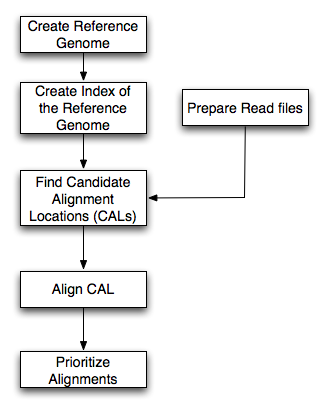
\includegraphics[bb=0 0 300 400, scale=0.5]{figures/workflow.png} 


\begin{figure}
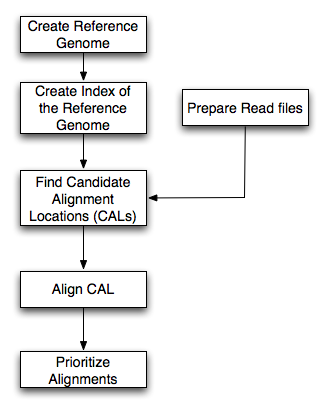
\includegraphics[scale=0.41]{figures/workflow.png} 
\caption{\small Overall workflow for a mapping procedure using BFAST
    (left). Description of BFAST subcommands and parallel and
    multi-threading execution capability (right).  In this work, we
    focus on the Candidate Alignment Locations (CALs) finding step due
    to its compute and memory intensive nature.}
\label{fig:bfast-summary}
\end{figure}


%  \label{fig:workflow-bfast}
% \capbtabbox{%
% \small
% \begin{tabular}{|c|c|c|c|} 
%   \hline BFAST & Description & Capable \\ command & & Parallelism
%   \\ \hline \hline \texttt{bfast fasta2brg} & creation of & multiple \\ &a ref. genome &
%   independent \\ & & contigs \\ \hline
%   \texttt{bfast solid2fastq} & preparation of & multiple sequence \\ & short
%   read files & read files\\ \hline

% \texttt{bfast index} & creation  & multi-threading \& \\
% & of reference  & low memory  \\ 
% &genome indexes&option \\
 
%   \hline
% \texttt{bfast match} & finding Candidate   &  multi-threading \& \\

% & Alignment &  parallel execution \\
% & Locations (CALs) & \\\hline
% \texttt{bfast localalign} & alignment of&   parallel execution \\
% &  each CAL   & \\

%   \hline
% \texttt{bfast postprocess} & prioritization   &  parallel execution \\ 
% & of alignments & \\
% \hline


% \hline
% \end{tabular}

% }{
% %  \caption{Description of BFAST commands and features for parallel and multi-threading execution. 
% %Note that the low memory option available for 'bfast index' does not target the parallel implementation directly, 
% %but this option could be utilized for task parallelization using low memory computing resources.}
% % \label{table:bfast-summary}
% }
% \end{floatrow}





%\begin{table}
%\small
%\begin{tabular}{|c|c|c|c|} 
%  \hline BFAST & Description & Features for \\ command & & Parallelism
%  \\ \hline \hline \texttt{bfast fasta2brg} & creation of & multiple \\ &a ref. genome &
%  independent \\ & & contigs \\ \hline
%  \texttt{bfast solid2fastq} & preparation of & multiple sequence \\ & short
%  read files & read files\\ \hline
%
%\texttt{bfast index} & creation  & multi-threading \& \\
%& of reference  & low memory  \\ 
%&genome indexes&option \\
% 
%  \hline
%\texttt{bfast match} & finding Candidate   &  multi-threading \& \\
%
%& Alignment &  parallel execution \\
%& Locations (CALs) & \\\hline
%\texttt{bfast localalign} & alignment of&   parallel execution \\
%&  each CAL   & \\
%
%  \hline
%\texttt{bfast postprocess} & prioritization   &  parallel execution \\ 
%& of alignments & \\
%\hline
%
%
%\hline
%\end{tabular} \caption{Description of BFAST commands and features for parallel and multi-threading execution. 
%Note that the low memory option available for 'bfast index' does not target the parallel implementation directly, 
%but this option could be utilized for task parallelization using low memory computing resources.}
% \label{table:bfast-summary} 
%\end{table}

In spite of the fact that BFAST has by design been made suitable to
exploit the computing capabilities of a range of modern processor
architectures, it is valid to ask if there remains other bottlenecks
(eg data flow/access) in the utilization of such architectures?
Additionally, if the answer is found to be positive, it is natural to
ask whether appropriate runtime environments can be developed in order
to overcome these limitations, and to enable BFAST's effective use of
distributed architectures?


% \begin{figure}
%  \centering


% 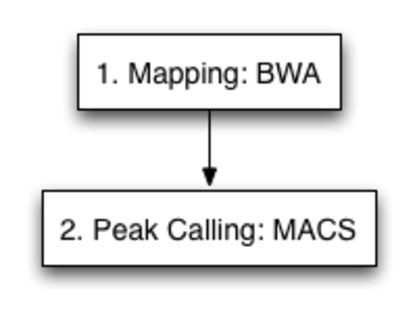
\includegraphics[bb=0 0 300 300, scale=0.39]{figures/chip-seq.pdf}

% \caption{\small Overall workflow of the ChiP-Seq pipeline.}
%   \label{fig:chip-seq} 
%  \end{figure}



\subsection{Characterizing BFAST: Computational and Data Requirements}


\begin{figure}
 \centering
%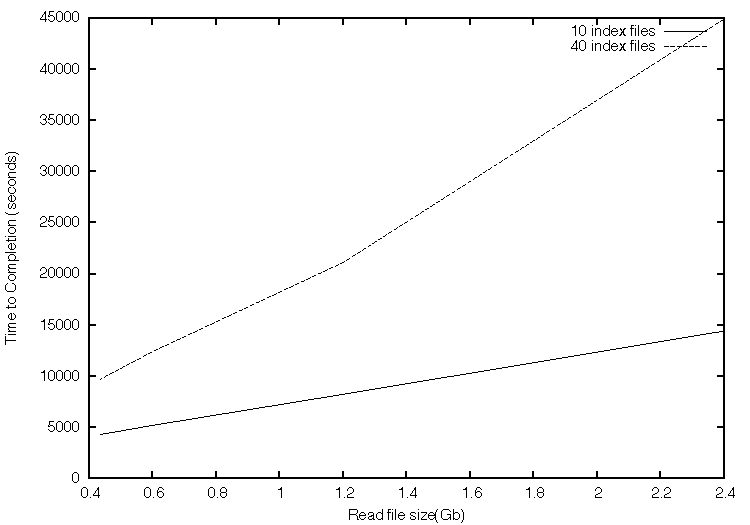
\includegraphics[bb=0 0 300 300, scale=0.55]{figures/readsvstime_hg18.pdf}
%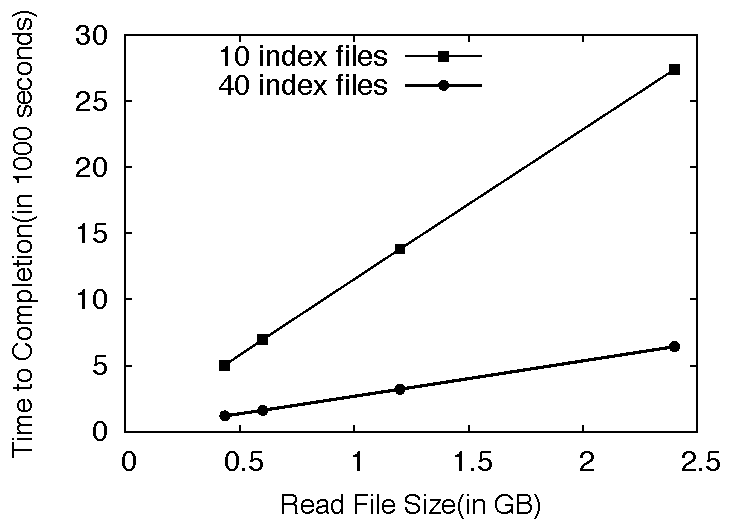
\includegraphics[bb=0 0 300 300,scale=0.55]{figures/readsvstime_hg18_chr21.pdf}
%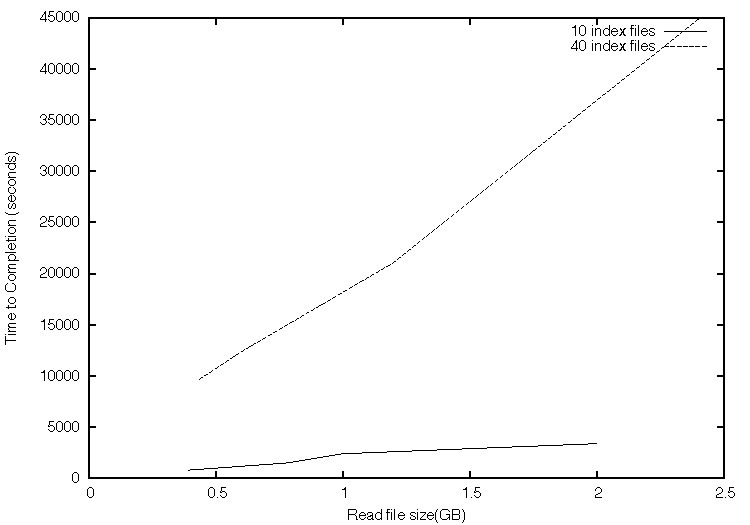
\includegraphics[bb=0 0 300 300,scale=0.55]{figures/readsvstime_bglumae.pdf}

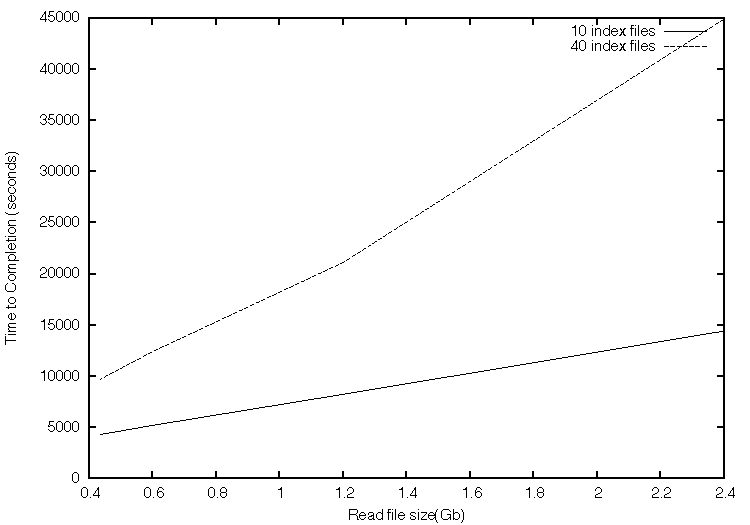
\includegraphics[bb=0 0 300 300, scale=0.42]{figures/readsvstime_hg18.pdf}
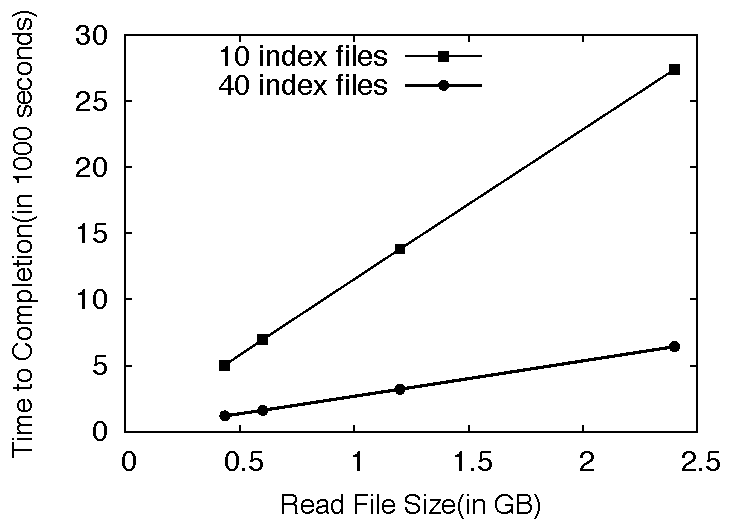
\includegraphics[bb=0 0 300 300,scale=0.42]{figures/readsvstime_hg18_chr21.pdf}
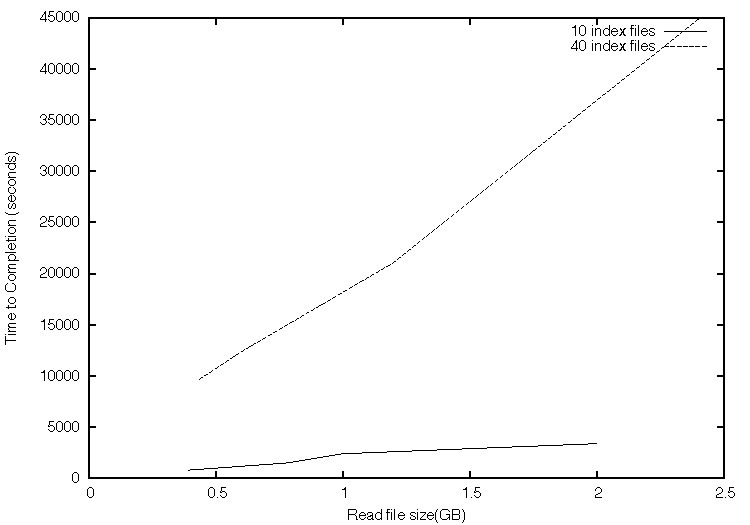
\includegraphics[bb=0 0 300 300,scale=0.42]{figures/readsvstime_bglumae.pdf}
%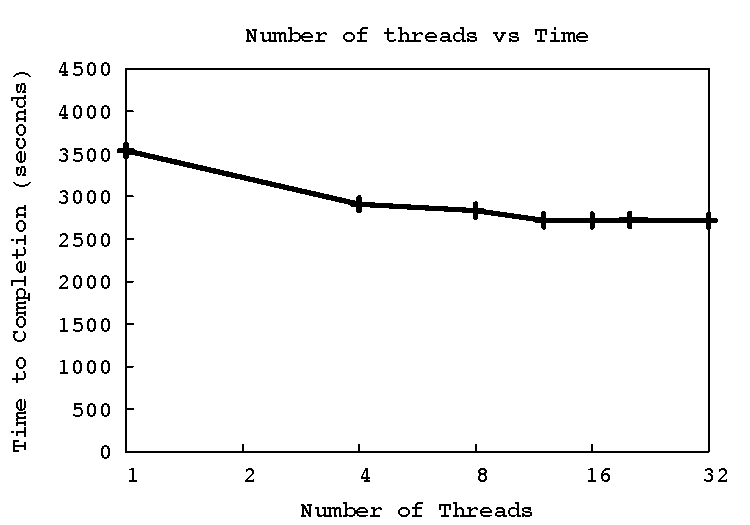
\includegraphics[scale=0.66]{figures/threadsvstime.pdf} 

\caption{\small The time-to-completion of the 'bfast match' step is
  measured by varying the size of short read files.  Two lines
  represent two cases differing in the low memory option, which
  results in the different number of index files (40 vs 10).  Results
  against the entire human genome (hg18) (upper) and chromosome 21
  only (middle) as reference sequences for exome analysis, are
  presented along with results with B. Glumae (lower).  The number of
  threads with the multi-threading option is set to 12. \jhanew{we
    discussed modifying these figures? E.g., the y-axis label of 2nd
    and 3rd sub-figures are over-running} }
  \label{fig:parallel-execution} 
 \end{figure}

\reviewer{R2 : Figure 2 should be done on the whole human genome too to compare the scalability.}



\begin{table}
\small
\begin{tabular}{|c|c|c|c|} 
  \hline 
Genome (Release ID)   & Human (hg18) & B. Glumae (BGR1) & Mouse (mm9)  \\    
   
\hline \hline
\underline{Reference Genome} & & & \\
    \# of Base Pairs (bp) &  3 Gbp & 7.3 Mbp & 2.6 Gbp\\ 
   Genome Structure &   23 (pairs of chr)  & 2 (chr) \& 4 (pl) & 21 (pairs of chr)   \\   
 
      \hline \hline
  \underline{NGS Data} & &   & \\
      Type of  Analysis &  Exome Analysis &  Resequencing & ChIP-Seq\\ 
  
          Sequencing Platform & ABI SOLiD  &  Illumina GA2 & ABI SOLiD \\ 
          Read Length & 50 bp & 36 bp & 36 bp \\

  Sequencing Data (fastq)  & 8.7 GB & 5.4 GB & 5.7 GB (treat) \& 6.5 GB (control) \\
  
  
  \hline  \hline
  \underline{BFAST} & &  & \\
  Minimum Disk Space &  approx. 200 GB   &    approx. 30 GB  &  approx. 84 GB (chr 19)\\
   Index Files Volume  & approx. 128 GB  & approx. 0.447 GB  & approx. 3.1 GB (chr 19)\\ 
\hline  \hline
\end{tabular} \caption{The summary of genomes, NGS data, and required disk space for running BFAST.  Mouse genome used for ChIP-Seq data analysis is converted in nucleotide space in spite of the fact that sequencing data were obtained with ABI platform.  For ChIP-Seq, two short reads data sets (control data and treat) are needed.  All read data are single-end.}
 \label{table:two-genomes} 
\end{table}

%\jhanote{This paragraph does NOT belong here! Place appropriately}
%First, performance gains with multi-threading are marginal showing
%only 30 \% speed up when reaches the limit with all of the number of
%free cores being used.  Also, it is apparent that the option has a
%limitation only until the number of required thread becomes equal to
%the total available cores in a given system, 12 cores in the case of
%results in Fig.~\ref{fig:parallel-execution}.

Before we can propose a scalable, extensible infrastructure to support
data-analytics on a range of problem-instances, it is critical to
characterize the computational and data dependencies of the BFAST
application.  The overall execution of BFAST, or any other short
mapping application that aligns short reads onto a reference genome is
affected by the specific biological problem at hand -- such as types
of target reference genomes and high-throughput sequencing techniques
and protocols, as well as computational attributes such as data
structure and formats and the ability to exploit the underlying
architecture.  Here, we present our investigation to characterize the
target application and more importantly the utilization of such
aspects with available computing architectures with respect to
parallel execution capabilities and data management.

\subsubsection{Computational Requirements for BFAST}

% It is important An understanding of computational requirements for
% carrying out BFAST steps is critically important for an infrastructure
% development that provides a way to execute the target genome-wide
% analysis tool with scalable distributed architectures.

In Table~\ref{table:two-genomes}, we summarize the typical values of
the parameters upon which the time-to-completion ($T_C$) typically
depends; values for two genome datasets that are representative of
biological diversity, an eucaryote system, human, and a microbe,
Burkerholderia Glumae\cite{kim2011} are listed. The two genomes differ
in the size and the genome structure of reference genomes, and types
of sequencing protocols.  Importantly, the two different genomes
display widely different data sizes in terms of the reference genome
sequence, short reads data, and required disk-space for carrying out
the mapping with BFAST.

% \jkimnote{The following four sentences were changed for describing new
%   results with Fig. 2}

To investigate the computational requirements, we first measure the
time-to-completion for 'bfast match' step while varying the size of a
read file.  The results are shown in
Fig.~\ref{fig:parallel-execution}. % \jhanote{This is pointing to the
% wrong figure?!}\jkimnote{fixed} 
Here, we present the time to completion ($T_C$) of exome analysis with
two different reference genomes, the entire human genome (hg18) and
one of its chromosomes, chromosome 21 (hg18-chr21), along with the whole genome
resequencing with a microbe, B. Glumae\cite{kim2011} (see Table~\ref{table:two-genomes}).  For
each case, we compare two different options for the \texttt{-d} flag.

As shown in Fig.~\ref{fig:parallel-execution}, time-to-completion 
scales linearly as the size of read files increases.
This suggests that if the read files can be broken up into smaller
fragments and which can be processed concurrently, there is the
possibility of a speed-up. This points to the potential of task-level
concurrency.

% indicating the parallel option with multiple read files is a useful
% strategy of scaling out, i.e.  using more cores with a smaller size
% of read files.

Secondly, the memory option ($d=1$) for generating 40 index files
(factor of four increase in the number of files\jhanote{4 difference
  in what?} compared to the option with $d=0$) indicates that there is
approximately a factor of four difference in the time-to-completion.
We calculated the ratios of slopes between 40 and 10 index files and
those are 3.50 (hg18), 4.25 (hg18-chr21), and 4.46 (B. Glumae),
respectively.  \jhanote{Previous sentence needs attention too}
Although many factors including the complex structure of the index
files affect on the speed-down with the option ($d=1$), the main
reason is that such low memory option requires four sequential CAL
finding with four index files as indicated in the
publication\cite{bfast2009}.  Therefore, this represents a classic
memory-time trade-off: in other words the peak memory consumed is
dependent on the size of the index files (which decreases as the
number of index files increases), whilst the runtime is dominated by
the size of the read-file (linear dependence).

Finally, we observed that the entire human genome required only two fold increase in $T_C$ compared to the mapping calculation with its chromosome 21.  These results suggest that unlike the task-level concurrency with read data, the task-level concurrency using biological information, i.e. independent mapping with individual chromosomes or plasmids is not a good choice in general. However, we note that disk space and memory requirement in some cases prohibit the use of a large reference genome.  For example, the human genome requires about 200 GB disk space and 16 GB memory and in fact, a small cluster of LONI (see Table~\ref{table:two-systems}) such as Painter cannot be used with the whole human genome as a reference genome.   In such cases, the task-level concurrency with biologically independent reference sequences might be a solution.   Overall, three cases shown in
Fig.~\ref{fig:parallel-execution} highlight diverse biological
contexts along with computational requirement of BFAST, leading to different optimal strategies for distributed
parallel executions.

% Secondly, the low memory option that creates more index files require
% a longer calculation time as found with the comparison between 40
% index files $(d = 1)$ vs. 10 index files ($ d = 0 $) ($n_m = 10$ is
% used).


% \jhanote{Joohyun: Please organize each description addressing each of
%   the following points: (i) Brief outline of the scientific problem,
%   (ii) What are the challenges, (iii) estimates of volumes of data
%   involved, distributed or not?, number of tasks, are they coupled or
%   uncoupled -- what is the level of coupling between tasks?}


% \begin{table}
 %\begin{tabular}{|c|cc|} 
 %\hline 
%Distributed &  HPC Grid &  Cloud \\ 
%Environment && (Eucalyptus)\\
%\hline
% &  Louisiana Optical & FutureGrid \\
%& Network Initiative  & \\
%System  Name &  QB/Small Linux Clusters   &  INDIA/SIERRA \\
%Disk Space  Limit  &  QB : unlimited  &    \\
%                         &  Small Linux Clusters : 100 GB  &  \\
 %\hline
 %\end{tabular}
%\caption{Specification of two distributed environments.  \jkimnote{need to fill Cloud systems}}
%\label{table:two-systems} 
%\end{table}
 
\subsubsection{Characterizing Data Requirements for BFAST}

% \jhanote{Table reference numbers still need fixing!!}\jkimnote{I fixed it what I saw. If I miss to fix some, this can be easily fixed since the location of 'label\{...\}' should be just before 'end\{table\}' in tables}

%The Table~\ref{table:dynamic-diskspace} dynamic disk-space required
%during the runtime of bfast match step.  As can be seen from the
%Table, the disk-space required for each read file is constant for a
%given size of read file.


\begin{table}
 \begin{tabular}{|c|c|c|c|c|c|} 
 \hline 
Case &Read& Index& Size of&  \# of & Approx.  \\
 &Files &  Files  & Temp File & Temp Files & Disk-space\\
 \hline
I&40 & 40 &105MB & 16 &67 GB \\
II&20 & 40 & 220MB & 16 &70 GB \\
III&40 & 10 & 105MB & 13 &52 Gb \\ 
 \hline
 \end{tabular}

 \caption{Table showing the required disk-space for operating data,
   for varying number of read files and index files, when all the read
   files are processed concurrently.  Number of concurrent tasks are
   equal to number of read files. The reference genome used is Human
   Genome 18 Chromosome 21 with total index file size 1.9 GB of and
   total size of read files was 8.9 GB.}
    \label{table:dynamic-diskspace} 
\end{table}

% The disk space required concurrent run of several read files in
% matching phase is important because if the amount of disk space
% required exceeds the available limit bfast fails. This plays a major
% role in determining the distribution of computation data depending
% upon the allowed disk space on each machine.

% The disk space required in concurrent run of several read files in
% matching phase is important because if the amount of disk space
% required exceeds the available limit bfast fails. This plays a major
% role in determining the distribution of computation data depending
% upon the allowed disk space on each machine.

% \jhanote{Lines 86-87, In a nutshell: the operating data-set does not
%   depend on the size/number of read files but does depend on the
%   size/number of index files. Needs to be explained.}

Generally speaking, mapping with BFAST should deal with the data for a
reference genome, short reads, and processed data generated in each
step.  Particularly, the temporary data generated during 'bfast match'
step needs careful attention due to their significant size and more
importantly a characteristic aspect such that the size depends on how
the step is executed, for example, concurrently vs. serially, or
centralized storage vs. distributed storage, or the low memory option
(i.e. the number of index files).

We estimated the peak disk-space requirement.  As shown
in Table~\ref{table:dynamic-diskspace}, the number of temporary files as
well as the size of each temporary file change depending upon the set
up for 'bfast match' step such as the number and the size of each read
file and the low memory option.  The low memory option changes the number and the size
of each index file, and thus temporary files are differently generated correspondingly.  For example, cases I and II that
are with $d=1$ and 40 index files require more space with more
temporary files than case III with 10 index files ($d=0$) does. Case
II need a bit more space than case I that is conducted with a half
number of read files but twice size of each read file.  In summary, our estimation on dynamically required disk-space with human
genome chromosome 21 suggests that the data volume would be a major
issue for a large genome system.
   
% Generally, fragmentation of data setsq is a primary idea to mitigate
% storage requirement as well as computing time.

% For example, as we mentioned above, separating short reads into
% multiple files is a good option with distributed computing
% resources.

Information on the overall data requirement is found in
Table~\ref{table:two-genomes} and
Table~\ref{table:dynamic-diskspace}. As mentioned, separating short
read data into multiple files (fragmentation) supports concurrent task
execution.  While a reference genome index should be treated as a
whole, there exists the possibly to break a reference genome.  For
example, breaking a reference genome into many independent sets is
possible, considering the fact that many organisms are composed of
independent parts, for example, chromosomes and plasmids or that
possible multiple contigs that represents discontinued genome
sequences would exist as a reference genome; the Human genome is a
fine example of this.
 %  Indeed, the human genome in
% Table~\ref{table:two-systems} with huge data volume as a whole is the
% case that combining ideas to split the target genome with all possible
% options ranging from biology to computing technologies is needed to
% overcome challenges arising from the data volume and computation.

\begin{table}
\small
\begin{tabular}{|c|c|c|c|c|} 
\hline 
Computing & Organization & System &  Storage & Disk-space  \\
Environment & & Used & Type  &  Limit \\ \hline
HPC Grid & LONI & QB & Disk & 58 TB   \\
 &  &  Painter/Eric  & Disk &  100 GB  \\
Cloud & FutureGrid & INDIA & Walrus & 230GB \\
         &                    &  SIERAA & Walrus & 58GB \\ 
Workstation &  Local   &  Cyder & Disk       & 5 TB\\

 \hline


 \end{tabular}
\caption{Specification of two distributed environments. LONI represents Louisiana Optical Network Initiative\cite{loni}. FutureGrid Cloud\cite{futuregrid} employs Eucalyptus}
\label{table:two-systems} 
\end{table}


%%\begin{figure}
% \centering
% 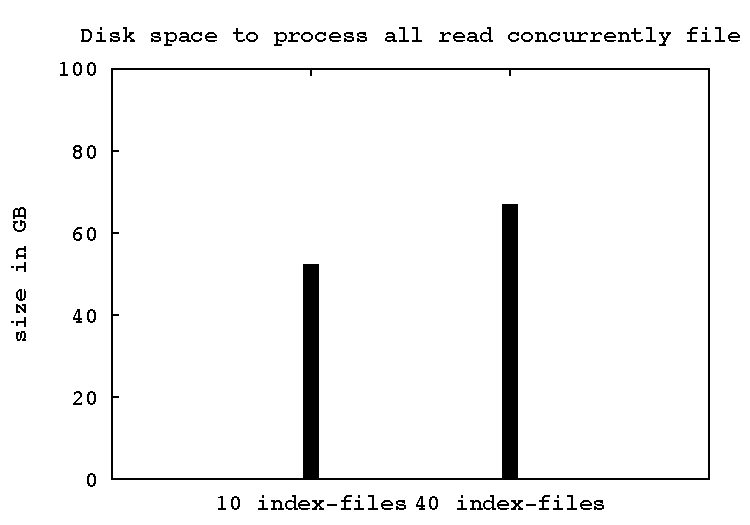
\includegraphics[scale=0.66]{figures/diskspace.pdf}
%\caption{\small Disk-space requirement for the cases that all read
%  files are processed concurrently in a single storage. 
%}
%  \label{fig:diskspace} 
% \end{figure}


\subsection{ChIP-Seq Pipeline: An example of Type II Application}

\begin{figure}
 \centering
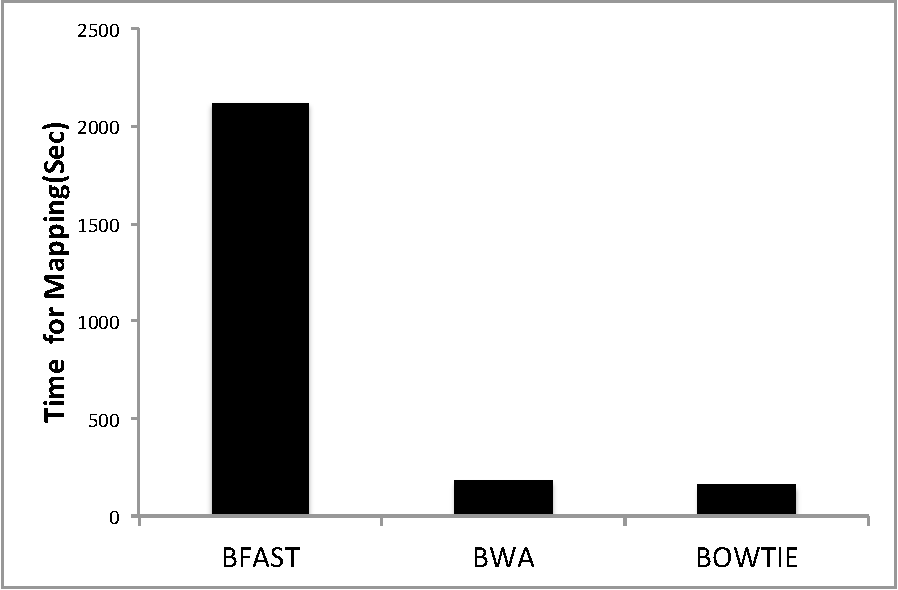
\includegraphics[scale=0.46]{figures/chip-seq-mapper-dependency-ttc.pdf}
\caption{\small Comparison of time-to-completion for the mapping step with three different mappers.  BFAST, Bowtie, and BWA were used. The file size of 100 MB short reads is used. \jhanote{Move
  left figure to section 2.4} 
}
  \label{fig:chip-seq-comp} 
 \end{figure}
 
The ChIP-Seq experiment provides genome-wide mapping of DNA-protein interactions, and obtained information is directly associated with transcription regulation\cite{pepke2009, laajala, wilbanks}.  An understanding of transcription regulation is one of fundamental goals in biological sciences because of its significance for virtually all aspects of biological processes in a living cell responsible for cell
development, differentiation, host-pathogen interactions, epigenetics,
tumorigenesis.  New drug or bio-marker discovery for many devastating diseases including
neurodegenerative disorders are examples of significant outcomes from such studies\cite{pepke2009}.  Replacing
ChIP-ChIP methods based on micro-array approaches quickly, the ChIP-Seq experiment became a main player with its genome-wide scale information and higher resolution.  ChIP-Seq means Chromatin Immunoprecipitation
(ChIP) followed by sequencing (ChIP-Seq), and thus the sequenced reads indicate the location of the peak where regulatory proteins bind with enrichment of reads. Generally, the conventional computational task
for ChIP-Seq is composed of two independent steps (see
Fig.~\ref{fig:chip-seq}).  In the first step, the mapping of two data
sets, corresponding to the control and the treat data, are carried out
separately, and in the second step, a peak caller, which carries out
statistical analysis to infer true peaks indicating DNA-protein
interaction regions, is executed.  The control data facilitate the construction of a peak model and background calibration, but it is optional. The unknown statistical nature of mapped reads, accompanied with errors arising from ChiP-Seq experiment process, along with the difficulty of increasing sensitivity in the mapping step due to the short length of reads (mostly up to 100 something at the time of this work) make the prediction of true peaks challenging\cite{pepke2009,laajala,wilbanks}  In this work, we use
the well-proven peak caller, MACS\cite{macs} for the second step, while three
different software tools, BFAST, Bowtie, and BWA, are employed for the first
mapping step.  These mappers differ in many ways, in particular with different computational requirements.  Two additional mappers, BWA and Bowtie are widely used due to their adoption of the memory efficient algorithm, Burrow-Wheeler Transformation, whereas BFAST was found to provide increased sensitivity\cite{bfast2009,mapping-survey}.  As shown in Fig.~\ref{fig:chip-seq-comp}, two mappers, BWA and Bowtie takes considerably shorter times compared to BFAST.  Note that the results presented in Fig.~\ref{fig:chip-seq-comp} were obtained by conducting the pipeline in which concurrent execution of the mapping step using 256 cores of a HPC cluster was managed.  Our main focus with the ChIP-Seq pipeline is to present a
compelling example how the use of scalable distributed infrastructure
as well as the runtime environment supporting dynamic execution of the
pipeline for ChIP-Seq data analytics leverage this powerful protocol utilizing NGS technologies. 

\section{NGS Data Analytics using Distributed, Scalable Architectures}

\jkimnote{this section should be revised including some benchmark number(s) with ChIP-Seq pipeline execution}


%\subsection{Existing Solutions: Limitations and Challenges}

% \jhanote{Here we need to define what solutions are currently employed,
%   what works well what doesn't}

%\begin{itemize*}
%\item GATK\cite{gatk}
%\item CloudBurst\cite{cloudburst}
%\item CouldBlast\cite{cloudblast}
%\item SNP finding and RNA-seq with Cloud\cite{langmead2009, langmead2010}
%\end{itemize*}

% Such solutions have demonstrated meaningful advances, and most of them
% have focused on the utilization of emerging technologies such as Cloud
% computing or the employment of algorithms for distributed computing
% such as MapReduce. 

% have garnered significant attention in particular 

\reviewer{R2 : CloudBurst is worth comparing with BFAST}

While interesting progress has been made in the algorithmic domain and
there exist efforts at providing a runtime environment to support,
some important requirement are notably missing in existing
infrastructural solutions. Most significantly, is the limitation that
most solutions are tailored for a specific problem instance. But can
an infrastructure be designed such that: it meets the requirements of
a large range of problem instances -- both in terms of size of data
involved and amount of computing required.  In order to meet these
requirements, the ability to utilize multiple and heterogeneous
resources will be inevitable.

There has been significant recent efforts in utilizing emerging
distributed computing environments such as clouds for genome-wide
analysis and infrastructure development
efforts\cite{taylor2010,cloudburst, cloudblast, langmead2009,
  langmead2010,gatk, halligan2009,luyf-2010}.
A general purpose infrastructure has also been extensively developed,
providing a variety of tools for genome-wide analysis through a
uniform interface or framework software\cite{galaxy}.


% For example the ability to utilize heterogeneous computing resources
% efficiently and effectively needs to be carefully addressed due to
% major efforts for building, maintaining, and extending an
% infrastructure.
% One interesting idea to mitigate such efforts is to make an
% infrastructure with a framework that is agile in dealing with
% heterogeneous computing and data management resources that are
% distributed geographically.  The agility should address a quick
% development cycle for an incorporation of a new bioinformatics
% application, an efficient maintenance of existing applications, and an
% easiness of addition of new applications or of extension of the
% infrastructure itself.  Additionally, one aspect, which is largely not
% considered in many existing solutions, is a way to enhance a target
% application with the utilization of heterogeneous scalable resources,
% for example, supporting task level parallelism without an intrusive
% modification of a target application and leveraging data management
% with a given data storage architecture.

% 
%%\begin{enumerate}
%\begin{itemize*}
%\item Agility for heterogeneous computing architecture
%\item Extensibility and quick development cycles for a new bioinformatics tool
%\item Scalability with a non-intrusive execution of a target tool  
%%\end{enumerate}
%\end{itemize*}


\subsection{Dynamic Application Runtime Environment}

We have established that efficient analytics on NGS data is not just a
matter of data-management, but also of providing large amounts of
computing for analysis. Any solution that facilitates analytics across
different problem instances, will require a general purpose framework
that is able to exploit different types of architecture and platforms.


%Given the large size of data involved, such as the as human genome as
%summarized in Table~\ref{table:two-genomes} and corresponding long
%computing times when carried out with a single or moderate size of
%clusters, parallel/concurrent execution of the target analysis with
%BFAST are desirable.
 
This could involve supporting fine-grained parallelism, of the type
that is supported by invoking the multi-threading option of BFAST, or
it could involve invoking multiple instances of BFAST executing
independently but on different read-files associated with the same
problem instance. Which approach will be more effective depends upon
the specific configuration of the problem instance, i.e., a problem
instance maybe I/O bound or compute/memory bound.

To achieve the goal of supporting both types of parallelism, on
heterogeneous distributed computing resources, we have developed the
Dynamic Application Runtime Environment (DARE)
framework\cite{dareurl,dare-tg11,dare-ecmls11}.

At the core of the DARE framework, is a SAGA BigJob (which is a
flexible general purpose pilot-job
implementation)\cite{saga-ccgrid10,saga-royalsoc,saga-web,jha2009developing,ecmls10}.
% Additionally, the framework is composed of a web application using an
% open source web development framework, Pylons\cite{pylonsurl}. 
% This
% combination of the open source technology and the application
% management system 
With a suitable Web development framework, it supports the development
of a lightweight but extensible, science gateway capable of using a
range of distributed resources.  In subsequent sections, we will
demonstrate via performance numbers the effectiveness of how the DARE
framework supports a range of infrastructure, problem instance
configurations and size.

Such task-level concurrency supports different ways of splitting the
data, whilst using the same runtime environment using SAGA-BigJob; all
the parallel tasks of BFAST steps are defined as sub-jobs in BigJobs.
It is possible to exploit multi-level configuration in that different
thread/cores configurations are possible for each of the sub-jobs.

\subsection{Understanding BFAST on a Local (Single) Resource}
\subsubsection{$T_{C}$ on $N_t$ and $N_c$}

To determine how the performance of the bfast match step varies with
the different number of threads, $N_t$, and cores, $N_c$, we measure
the time-to-completion, $T_C$ of a task of the bfast match step on a
single machine having multiple cores.  As shown in
Fig.~\ref{fig:threading-benchmark}, $T_{C}$ indicates a speed-up until
the number of threads becomes equal to the maximum number of cores.
Interestingly, the overall performance gains about 30 \%, and the
scaling tendency does not reveal any strong pattern but a weak
log-linear behavior. 


%... \jhanote{needs merging} The results from our investigation are presented in
%Fig.~\ref{fig:parallel-execution}. First, performance gains with
%multi-threading are marginal showing only 30 \% speed up when reaches
%the limit with all of the number of free cores being used.  Secondly,
%the multiple read file option is useful as a strategy for scaling out,
%i.e. with more cores operating correspondingly a smaller read file.
%Thirdly, the low memory option that creates more index files require
%longer calculation time as the comparison between 40 index files $(d =
%1)$ vs. 10 index files ($ d = 0 $) and $n_m = 10$.
%
%
%... \jhanote{needs merging} Computational requirements vary also with
%how to configure parallel/multi-threading execution patterns.  Since
%BFAST provides its intrinsic support for multi-threading and parallel
%execution, we examined computational requirements while varying
%configurations for such parallel strategies.  For example, according
%to the results shown in Fig.~\ref{fig:parallel-execution}, it is
%obvious that dividing a large volume of short reads data into many
%independent runs is a good strategy while multi-threading support is
%limited by available cores in a same node.  Also the results in
%Fig.~\ref{fig:parallel-execution} find that the low memory option that


 \begin{figure}
 \centering
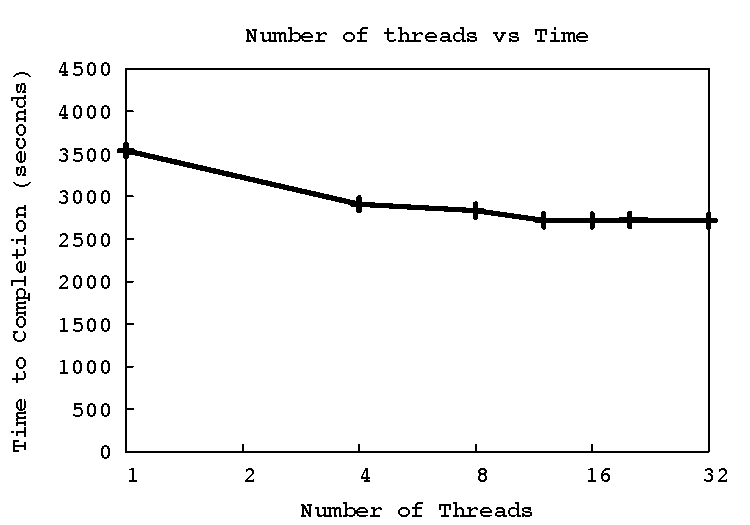
\includegraphics[bb=0 0 340 300, scale=0.39]{figures/threadsvstime.pdf} 

\caption{\small Measuring the time-to-completion ($T_C$) as a function of the
  number of threads.  The node (Cyder)used for tests has 12 cores.  Human
  genome (hg18) chromosome 21 is used as the reference genome. The low
  memory option with 40 index files is used for this measurement. The
  $T_C$ decreases logarithmically, till the number of
  threads is equal to the number of cores, after which the performance
  levels off. Similar behavior is observed for different machines
  with varying number of cores.}
  \label{fig:threading-benchmark} 
 \end{figure}

\subsubsection{Understanding I/O}

We conducted experiments with four different configurations, wherein
we varied the number of threads per task, and the number of tasks
running concurrently such that the total number of cores utilized at
any stage is fixed to the number available on the single node -- 4
(see Table~\ref{table:understandio}) The total amount of short-data
processed per task varied such that the total amount of short-date
processed was a constant.

Case s1 provided the starting configuration where 1 (BFAST) task was
run with 4 threads; in subsequent configurations (s2 and s3) the
number of tasks were increased (up to the number of cores available),
with a concomitant decrease in the threads per tasks (so as to be
constant at 8). We find that although in general, $T_C$ decreases as
the number of tasks increase (s1 to s2) and thus the amount of
data-processed per task decreases, that is not universal. Specifically
in going from s2 to s3, there is an increase in the $T_C$.  The exact
cause for such behavour is unknown, but points to read-contention on
index files along with an I/O bottleneck.

% The comparison between s1 and s2 suggests clearly the
% configuration of s2 is more efficient to utilize task-level
% concurrency using a smaller size of short reads than the configuration
% with more threads in a task requiring a larger size of short reads.
% Considering the amount of total reads in these two experiments are
% exactly same, a noticeable difference in $T_C$ indicates the
% importance of finding an optimal configuration for a better
% performance.

In the case of s4, 4 bfast tasks were also run on a single node; the
performance was better than for s3. This can be expected because
although the four bfast tasks were trying to access the same set of
index files for processing, multi-threading option was used.  In this
case all LONI machines have a Lustre filesystem for accessing the
input data.  Because of increase in access of same files there has
been a unpredictable behavior in time-to-completion (s3). This was
also observed on other local server -- Cyder and Walrus (Eucalyptus
cloud storage) based systems.

% The comparison between s3 and s4 finds that a slight gain in the
% performance when more threads are utilized per a task.


% Finally and interestingly, the results s3 and s4, compared to s2,
% indicates the significance of I/O for an optimal configuration since
% two cases require more memory due to the larger volume of short read
% data.\jkimnote{not sure this is correct}

% The system I/O influences the performance of the step for finding CALs
% (bfast match).


 \begin{table}
 \small
 \begin{tabular}{|c|c|c|c|c|c|} 
 \hline 
Case & Read File  & Threads & \# of   & $T_C$ \\
& Size &  per Task &  Tasks &   \\  \hline
s1 & 2.4 GB &  4 & 1 & 9358 s \\
s2 & 1.2 GB & 2 & 2 & 5290 s \\
s3 & 0.6 GB & 1 & 4 & 9152 s \\ 
s4& 0.6 GB & 4 & 4 & 5804 s \\

 \hline
 \end{tabular}
 
 \caption{Computing time for the 'bfast match' step on a single node
   (eric). Note that all cases have the same amount of total read
   data, and use ten index files.  Under the restriction that the
   hardware node has 4 cores, the time-to-completion is compared with
   varying conditions regarding the size of read files, the number of
   thread for each 'bfast match', and number of the 'bfast match'
   executed concurrently.  }
   %$V_r$ represents the total volume of short read files (equals to the number in the second column multiplied by the number in the fourth column), and thus $T_C/V_{r}$ is the ratio for a computing time per a data volume} & $T_C/V_{r}$
    \label{table:understandio}
\end{table}

%The experiment results in Table~\ref{table:understandio} show that use of 2 threads per bfast matches simultaneously 
%on a four core node is the optimal configuration for time to completion. Because it balances each thread per core but  
%running the two bfast jobs per node at the same time. Thus shows advantage of running multiple bfast matches simultaneously. 

%\jhanote{Lines 44-47 of the Excel Sheet here}





% First, biological information could be utilized for such parallel
% execution.  For example, the short read sequences in fastq format
% could be split into many files that are needed separately for
% parallel mapping.  At the last stage, all mapped results could be
% combined with available tools such as SAMTools\cite{samtools}.
% Additionally, a reference genome could be divided into many if each
% dataset contains independent contigs.  For example, each chromosomes
% or plasmids in microbes could be a separated sub-genome sequence
% contig.  However, note that indexes of an entire contig should be
% used together, regardless of the low memory option that allows to
% store indexes in many files, which is in fact the major obstacle to
% require a large disk-space.

%...\jhanote{needs merging} Most importantly, while the implementation
%of multiple parallel tasks indicates advantages of distributed
%multiple resource utilization, the large volume and variation of data
%sizes associated with genome sequence data as well as minimally
%required disk space needs to pay attention since in some cases, data
%size itself prohibits to carry out the analysis in a computing
%resource that lacks the demanded requirements, indicating the
%significance of agile runtime environment that drives a dynamical
%configuration and utilization of distributed resources.

\subsection{Execution of BFAST mapping on Distributed Resources}
% Grids and Clouds}

In order to demonstrate the flexibility of the DARE framework and its
ability to support both fine-grained parallelism and task-level
parallelism, over multiple cloud environments, we perform tests over a
HPC-grid (LONI) and a Cloud resource (FutureGrid) (see
Table~\ref{table:two-systems} for details of the infrastructure).


\subsubsection{Using BFAST on HPC Grids}

The first two configurations -- case g1 and g2 in
Table.\ref{table:bigjob-loni} demonstrate how the DARE framework can
support a large range task-concurrency without losing scalability.
Specifically, in g1 \& g2 all parameters and conditions are kept
similar, but the number of BFAST tasks (sub-jobs) are varied, and thus
the number of cores utilized.  The individual processing time of each
BFAST task is, as expected to decrease in proportion to the data-file
size; interestingly, as can be seen, with twice as many tasks
(sub-jobs) utilized within a BigJob, the time taken decreases by half,
i.e., the increase in the coordination cost of multiple BFAST tasks is
negligible. This provides a simple, but important test of scalability
(with the number of tasks) of the DARE framework.  

In cases g3 and g4, the number of BFAST tasks (sub-jobs) is greater
than the number of cores available at any one instance; thus multiple
generations of tasks have to be staged in as cores become available
(when earlier tasks finish).  For g3, six generations of tasks have to
be completed; comparing g3 with g1 there is an approximate factor of
six difference in $T_C$. Similarly $T_C$ for g4 is a factor of six
greater than g2 as would be expected if the coordination overhead of
staging in tasks was not too great. This suggests that the DARE
framework not only supports efficient concurrent task execution, it
also supports efficient execution over a range of BigJob/resource
sizes.

For g5 and g6 the number of index files is 10; to be contrasted with
40 for g1-g4.  However, in spite of a different index file number, the
linear scaling behavior exists.  As discussed in \S 2.2.1, the
time-to-completion depends has a linear dependence on the index files
(memory-time trade-off); once this is taken into account the total
time-to-completeness is consistent with g1-g4.


 \begin{table}
 \small
 \begin{tabular}{|c|c|c|c|c|c|} 
 \hline 
Case & Read File & Threads   &  \# of & BigJob Size   &   $T_C$   \\
   & Size& per Task & Tasks  & Cores(Nodes)  & \\
   \hline
g1 & 0.209 GB & 2 &   40 &  80(10) & 3966 s \\
g2 & 0.435 GB & 2 &  20 & 40(5) & 8031 s\\ \hline
g3  & 0.209 GB& 2 & 40  & 12(3) & 25807 s \\
g4 & 0.435 GB& 2 & 20  & 12(3) & 23872 s  \\ \hline
\hline
g5 & 0.209 GB& 2& 40 & 80(20) & 1111 s \\
g6&0.435 GB&2& 20 & 40(10)&2096 s\\
\hline
\end{tabular}
\caption{Performance comparison for different parallel configurations
  using SAGA-BigJob on a HPC-Grid (LONI). One BigJob is submitted with
  the number of sub-jobs, where each sub-job is a BFAST task.  The
  total (read) data size is the read-file size multiplied by the
  number of tasks (which is equal to the number of read-files); which
  is a constant for g1-g6.  Cases g1, g2 and g3,g4 and g5,g6 are
  conducted on QB, Painter and Eric respectively. The cases g1, g2,
  g3, g4 are use 40 index files of a Human Chromosome 21.  Note that
  g5 and g6 are the results with 10 index files; g6 is specifically
  carried out to provide a direct comparison to c5 (on a cloud
  resource as in the following Table~\ref{table:cloud-VM}) }
  
  \label{table:bigjob-loni} 
\end{table}

% \subsubsection{Using BFAST on Clouds}

% First of all, Table~\ref{table:bigjob-loni} presents the
% results of the time-to-completion, $T_C$ of the step 'bfast match'
% while varying different configurations that include the variation of
% the number of threads used for each task and the number of cores (and
% also the number of nodes) through a BigJob set
% up\cite{ecmls10,saga-ccgrid10}.  These results clearly show robust
% execution of job submission and SubJob management trough BigJob in
% spite of a large number of sub tasks up to 40 and multiple generations
% of concurrent tasks when the total number of concurrent tasks is
% limited.  The main finding of these experiments is, perhaps, that the
% best result with respect to $T_C$ can be achieved when sufficient
% numbers of cores for the total set of tasks are promptly available
% from distributed computing resources as indicated with the best
% performance with g1.  The comparison between g1 and g2 clarifies
% further this finding such that when all required tasks can be run
% concurrently using available cores, $T_C$ is roughly proportional to
% the size of each read file.  On the other hand, when the number of
% cores managed by BigJob is limited to execute the total number of
% tasks concurrently, like the cases of g3 and g4, BigJob needs to
% manage all tasks using multiple generations of concurrent tasks and
% therefore a longer $T_C$, roughly scaling with the number of
% generations required, results.  


\subsubsection{Using BFAST on Clouds}

\reviewer{R-7 : I don't buy the cloud argument in section 3.3.2
  because it avoids the fundamental issue in any data intensive task:
  data transfer between master and workers (or from a site to Amazon
  in the commercial setting).  The authors stress a flexible ** and
  scalable ** framework and there is no scaling for this on more than
  8 cores and no real clear evaluation of how a parallel file system
  (or lack thereof) fits into this clearly data intensive problem.
  There is little support for the statement in the abstract that this
  work "scales-up and scales out over production grid and cloud
  environments" as there are only two data points for scaling up data
  (that are very small relative to real data in Figure 2 depending or
  not if there was quality information inside) and cores (in the case
  of the cloud, looking at a few instances).  The real interesting
  question is the one they reserve for future work: data access
  mechanisms to the different types of storage, which is where the
  scaling in our experience always suffers beyond a few hundred
  cores.}

In the previous sub-section, we established the ability of DARE to
support concurrent task execution by establishing the scale-out to a
large number of cores/resources. Although we did not use physically
distributed resources to validate their performance, we used logically
distributed tasks and have in earlier work established performance
over distributed HPC grids\cite{saga-ccgrid10}.  The question that
therefore arises: can the DARE framework support similar capabilities
of scaling on clouds without sacrificing the ability to utilize
fine-grained parallelism as needed? We attempt to address this
question in the remainder of this section.

As mentioned, the cloud infrastructure used was the Eucalyptus based
IaaS resources on the NSF-sponsored FutureGrid\cite{futuregrid}.
Resource descriptions are summarized in Table~\ref{table:cloud-VM}.

Case c1 and c2 have the same workload, however c2 uses an instance
type c1.xlarge, whilst c1 uses a m1.large instance type.  In the case
of c1 four different BigJob agents on four VM's were launched, as
opposed to one BigJob agent on a single VM in case of c2.

For exactly the same workload, the $T_C$ for cases c1 and c2 are shown
in Table~\ref{table:cloud-VM}. We find that even though the number of
cores and number of BFAST tasks employed are the same (8 and 4
respectively), the $T_C$ for c2 is lower than that for c1; this is
because there exists an overhead of marshaling 4 BFAST tasks into 4
VMs compared to 1 VM.  Additionally, c1.xlarge is a more powerful
instance than m1.large. 

In contrast, c3 represents the configuration when a single large
instance (c1.xlarge) is used for a single BFAST instance but using
multiple threads; interestingly the $T_C$ is larger than c1 or c2.  We
attribute this to the fact that increasing the number of threads
increases the performance only logarithmically, whilst increasing the
number of concurrent tasks executed (c1 and c2) has a linear
performance improvement. The increase in $T_C$ for c3 now arises
due to the fact that the size of the read file that is
an important determinant of performance is now 4 times as larger
than c1 or c2.


% Here, we want to note that some difference in executing an
% application such as BFAST with a HPC grid and with a Cloud
% environment.  There exists a slight edge with a larger VM indicating
% the overall $T_C$ could be dependent on how to utilize available VMs
% and distributed the same work load across VM's.  Generally, a HPC
% system has a large size of disk-space that can be accessed from all
% computing nodes but sometimes there exists a restriction to utilize
% them.  For example, among LONI systems, the largest cluster, QB has
% a significantly large disk-space while small cluster systems such as
% Painter allows only 100 GB imposed by the administration policy (see
% Table!~\ref{table:two-systems}).  On the other hand, the Cloud
% environment we tested supports additional storage via the walrus and
% this storage can be accessed by all VMs utilized together.


% Although not very insightful, for completeness and and for pedagogical
% reasons it is instructive to compare grid versus cloud performance for
% identical work load configuration and resource capabilities.  We
% compare the result with g6 of Table~\ref{table:bigjob-loni} and the
% result with c4 of Table~\ref{table:cloud-VM}; they have a similar
% configuration with the same number of total tasks and cores, but c4
% has a lower $T_C$ than g6. In spite of the virtualization layer this
% is true probably because c1.xlarge uses newer and more powerful
% hardware than the 4 year old hardware of g6, as well as the fact that
% virtualization costs are a small percentage of overall costs for long
% running jobs (even if ``hot'' start-up times are significant).  A
% rigorous comparison would entail a comparison of data access
% mechanisms to the different types of storage on grids and clouds,
% which is beyond the scope of this current work.

% Nonetheless, the results presented in Table~\ref{table:bigjob-loni}
% and Table~\ref{table:cloud-VM} demonstrate the capability of the DARE
% framework to effectively utilize heterogeneous distributed computing
% resources.

% Generally, a HPC system has a large size of disk-space that can be
% accessed from all computing nodes but sometimes there exists a
% restriction to utilize them.  For example, among LONI systems, the
% largest cluster, QB has a significantly large disk-space while small
% cluster systems such as Painter allows only 100 GB imposed by the
% administration policy (see Table!~\ref{table:two-systems}).  On the
% other hand, the Cloud environment we tested supports additional
% storage via the walrus and this storage can be accessed by all VMs
% utilized together.  We do not compare how the data access mechanisms
% to these different types of storages affect on the choice of execution
% patterns, in particular, with a Cloud in this work, since we consider
% an understanding of such factors is beyond the scope of this work.
% Nonetheless, the results presented in Table~\ref{table:bigjob-loni}
% and Table~\ref{table:cloud-VM} demonstrate the capability of our DARE
% tool for the utilization of heterogeneous distributed computing
% resources.




%... \jhanote{needs merging} In the Grid implementation first all the
%data required in the steps was transferred to machine's work directory
%where we want to start the BigJob. The BFAST was installed in the home
%directory and the executables path for job description of SubJobs was
%given accordingly.

%... \jhanote{needs merging} In the cloud implementation all the data
%required was transferred into the walrus (Eucalyptus storage on Futuregrid) because of the data size
%limitation of the storage space in the running VM. Multiple VM's can
%be started at once and the data in the walrus was mounted onto all the
%running VM during its booting. Thus all the VM can have
%access to data and can process concurrently. VM should also include the installation of
%SAGA and SAGA-BigJob. Thanks to SAGA-BigJob for providing the flexibility of 
%handling grids and clouds together with the same implementation of BigJob.

%In Table~\ref{table:cloud-VM}with help of bigjob cloud implementation we designed two
%experiments. In the first experiment (c1) four  VM's of type $m1.large$ with 2 cores each were
%started and four bfast matches with one bfast on each one using SAGA
%bigjob . In the second experiment (c2) a large VM of type $c1.xlarge$ with 8 cores is started
%and 4 bfast jobs were launched on the same VM simultaneously using
%SAGA bigjob.

 \begin{table}
 \small
 \begin{tabular}{|c|c|c|c|c|c|c|} 
 \hline 
 Case&Read File&Threads  & \# of & Total & \# of  &  $T_C$  \\ 
     & Size  & per Task & Tasks & Cores &  VM's & \\ 
\hline

c1& 0.435 GB&2 &  4 & 8 & 4 & 1492 s\\
% 1495 +1487 
c2 &0.435 GB & 2 & 4  & 8  & 1 &1149 s\\ 
c3 & 1.74 GB &8 & 1 &  8 & 1 &4528 s \\\hline
\hline
c4 & 0.435 GB&2 & 20 & 40 & 1 &1137 s \\
\hline

 \end{tabular}

 \caption{ The number of index files used for this measurement is 10.
   In all cases the input and output data resides on VM itself.  VM in
   case c1 is of type m1.large whereas c2, c3, c4 are of type
   c1.xlarge }
  \label{table:cloud-VM} 
\end{table}

%\jhanote{Need to refer to Table\ref{table:cloud-VM}}

\subsection{The need of flexibility, extensibility, and scalability in a ChIP-Seq pipeline}

In Fig.~\ref{fig:chip-seq-comp-2}, we compare the number of predicted peaks using the developed pipeline with three different mappers.  These calculations were carried out without considering the control data and the reference genome sequence is Chromosome 19 of mouse genome (mm9).  We used the same peak caller, MACS for these calculations, and thus we found that peak calling results were considerably affected by a mapper.  We note that not only the number of predicted peaks but also significant difference in statistical quantities for predicted peaks such as False Discovery Rate was observed (not shown).  The resulting variation is in fact not surprising since the mapping results varies with a chosen mapper.   For example, we found that for the treat data, 8,375,179 reads were mapped by BFAST whereas 3,104,010 reads and only 277,427 reads were mapped by BWA and Bowtie, respectively, which is in accordance with findings by others and ours with different data sets\cite{bfast2009,mapping-survey}.  In fact, it is well known that different peak callers produced non-equivalent results and to some extent, practical validation of a software tool for peak calling is still non-trivial for ordinary researchers\cite{wilbanks, laajala}.  Here, according to our results, we find that the consequence of the mapping step is another factor affecting sensitivity of peak calling.

Varying results with different software tools and pipelines, and more importantly the difficulty of validation of peak calling procedure suggest clearly the need of flexible pipeline in which multiple alternative tools are utilized and the support of scalable executions for increased computing requirements is realized.  In our approach, using DARE-based runtime-environment, a target pipeline is efficiently built and runs on distributed infrastructures effectively.  
Our ChIP-Seq pipeline, implementing DARE-based Type II service, demonstrated a practical solution for pipeline approaches of NGS data. 

\begin{figure}
 \centering
%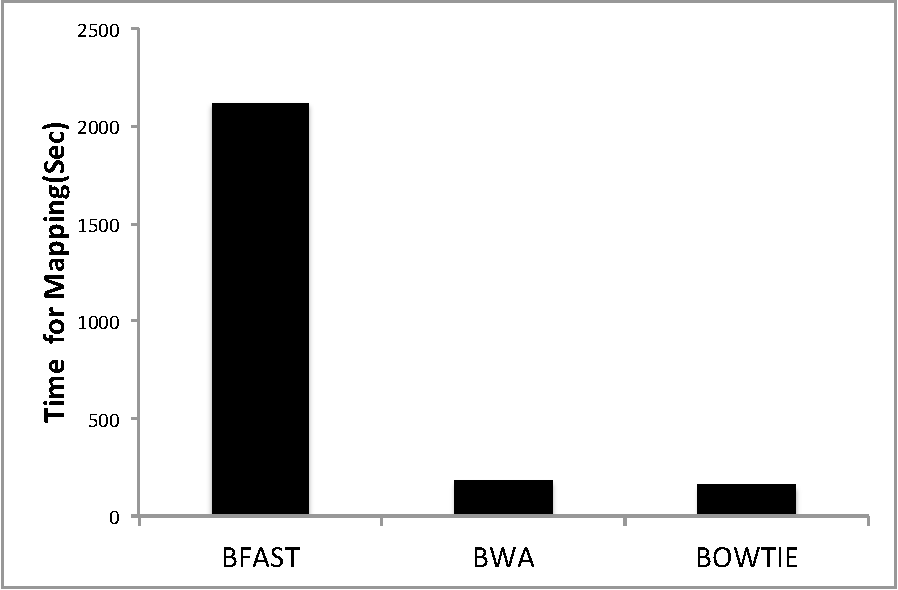
\includegraphics[scale=0.46]{figures/chip-seq-mapper-dependency-ttc.pdf}
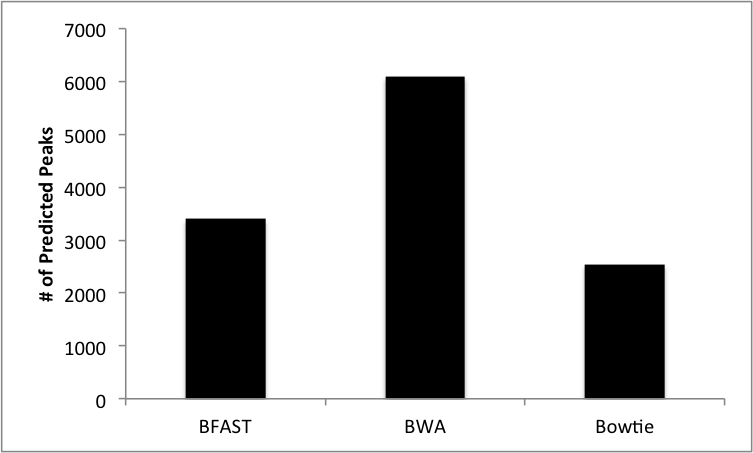
\includegraphics[scale=0.40]{figures/peaks_tool.png}

%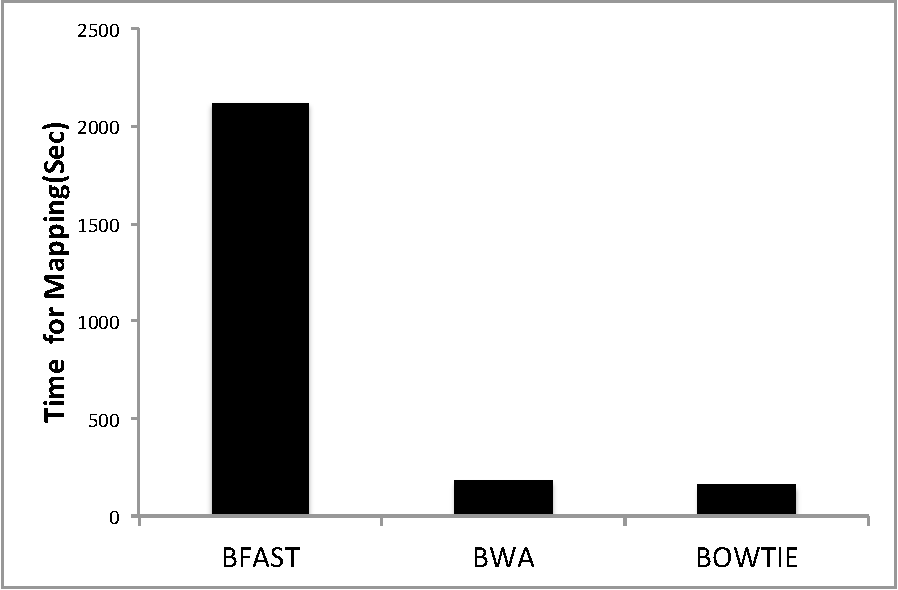
\includegraphics[bb=0 0 300 300,scale=0.39]{figures/chip-seq-mapper-dependency-ttc.pdf}
%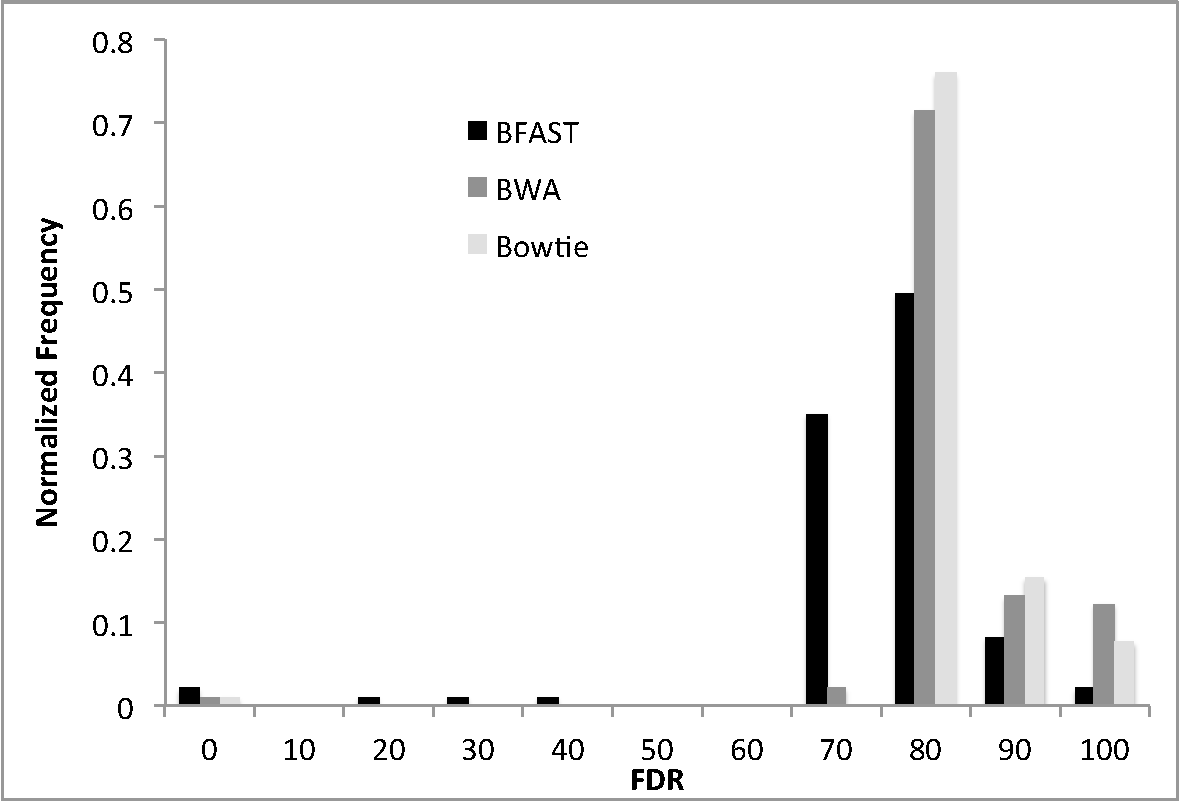
\includegraphics[bb=0 0 300 300,scale=0.30]{figures/chip-seq-mapper-dependency-results.pdf}
%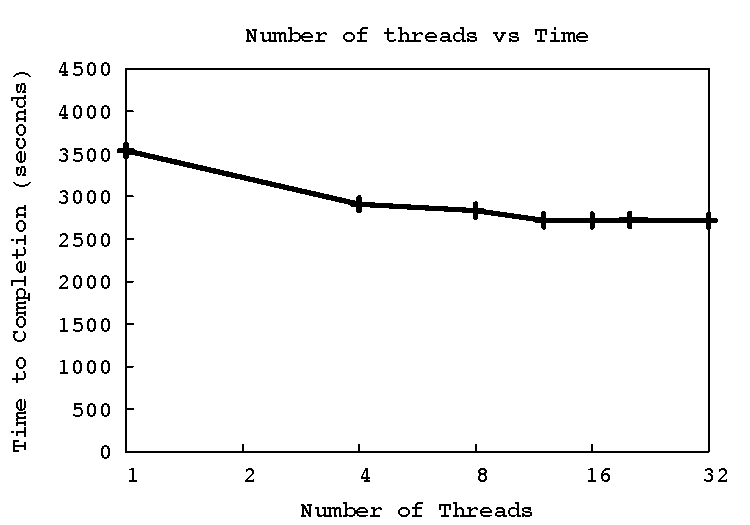
\includegraphics[scale=0.66]{figures/threadsvstime.pdf} 

\caption{\small % Comparison of results using different mappers for the
%   ChIP-Seq.  Time-to-completion for the mapping step is compared among
%   three different mappers, BFAST, Bowtie, BWA (left). \jhanote{Move
%     left figure to section 2.4} 
  Peak calling results are compared with the number of predicted peaks using different mappers for the first step.  For
  these calculations, the same treat reads data are mapped onto the chromosome 19 of mouse reference genome (mm9)}
  \label{fig:chip-seq-comp-2} 
 \end{figure}



\section{Conclusion and Future Work}

The challenges of Next Generation Sequencing are significant
and pervasive.
BFAST which has emerged as an important analytic tool for NGS, is  a sophisticated application that has the
capability to utilize advanced architectural features -- in particular
at the processor level, such as multi-threading and support for low
memory run-time configurations. However, by analyzing the human
genome, we find that more often than not, in order to perform analysis
at the scales required, additional support for concurrent execution is
required, whilst exploiting the fine-grained parallelism. We also
observed, that for BFAST -- which is a data-intensive application,
the performance bottleneck often becomes I/O; we establish that in
order to overcome the I/O induced bottleneck, any effective run-time
environment must support both scale-up and scale-out. In other words,
a sophisticated run-time environment for BFAST is required.

This paper represents the initial steps in the design and development
of a general-purpose, scalable and extensible infrastructure to
support next-generation (gene) sequencing data-analytics. To the best
of our knowledge the approach in this paper is unique in that we
analyze both the data-intensive and the computational requirements of
typical analytics performed on the data, which in turn motivates the
architecture and implementation of the infrastructure. 

We have analyzed the requirements which are valid for a broad spectrum
of problem instance sizes; however, we have demonstrated the
capabilities and effectiveness of our architecture for a reduced
problem instance. The immediate next step is to demonstrate the
effectiveness for larger problem instances, e.g., genome wide
variation studies with many individual human-genomes, through both the
scale-up and scale-out of the infrastructure.  Additionally, we will
extend our framework to develop and support multi-stage workflow,
i.e., the full pipeline,
 
We have begun implementing the next steps and features for this
project. In an attempt to provide these advanced capabilities to the
community, we are working on NGS Data Analytics Science Gateway that
will abstract many of the infrastructure details and provide
``autonomic'' capabilities, i.e., map the specific problem instance to
the appropriate backend infrastructure.

The mapping with BFAST and the pipeline discussed in this work are freely available via our gateway, DARE-NGS (http://dare.cct.lsu.edu).

% We present analyses with two genome systems representing a eukaryote
% and a prokaryote, respectively, using a HPC grid and a Cloud
% environment for an understanding of conditions of a scalable
% cyberinfrastructure for an effective execution of mapping, and
% consequently genome-wide analyses.  Based on our results, we conclude
% that an infrastructure to run with a proper configuration for
% concurrent tasks benefits genome-wide analysis and such a
% configuration is optimized only when parameters from biological
% contexts as well as limitations and potentials of distributed
% computational resources are taken into account together.  For that
% purpose, our DARE framework provides an efficient solution.

\section*{Acknowledgement}

The project described was partially supported by Grant Number
P20RR016456 from the NIH National Center For Research Resources.  We
also acknowledge Ole Weidner and Le Yan for useful performance related
discussions, Diana Holmes for sharing her experience with mapping
using BFAST, and Jong-Hyun Ham for allowing us to use B. Glumae genome
sequences.  \jhanew{JK -- please acknowledge Chris Giss} Computing
resources were made possible via NSF TRAC award TG-MCB090174 and LONI
resources.  This document was developed with support from the National
Science Foundation (NSF) under Grant No.  0910812 to Indiana
University for ``FutureGrid: An Experimental, High-Performance Grid
Test-bed.''

\bibliographystyle{abbrv} 
\bibliography{ecmls11}


\end{document}

Any opinions, ndings, and conclusions or recommendations expressed in
this material are those of the author(s) and do not necessarily
reflect the views.


% in addition to the requirement of an uderstanding of applications of
% interest in terms of the capability of parallel execution in
% heterogeneous computing environment,

% and importantly, difficulties of utilization of heterogeneous
% distributed computing resources

% This is partly because, in addition to requirement of an understanding
% of applications of interest in terms of the capability of parallel
% execution in heterogeneous computing environment, the complexity of
% biological contexts associated with characteristics of a target
% genome(s), the volume of relevant genomics data, and importantly,
% difficulties of utilization of heterogeneous distributed computing
% resources constitute challenges for introducing an appropriate
% scalable architecture for the infrastructure.

% required software is relatively less
% recognized for its significance.  

% The need of computational methods as well as computing architectures
% for compute-intensive and data-intensive calculations for resolving
% new challenges arising from requirements of processing and analyzing
% genome sequencing data, therefore, is regarded indispensable for
% accurate and reliable analysis against high-throughput sequencing data
% and following genome-wide analyses.

%% As a result, remarkable advances have been witnessed in recent years
%% and a number of bioinformatics tools aiming to solve emerging
%% challenges are currently available to the scientific
%% community\cite{trapnell2009,bfast2009,scheibye-alsing2009,pepke2009,samtools}.

% The need of such infrastructures is also understood with
% catastrophically growing datasets for genomics and their applications
% for public heath issues.

% Nonetheless, some interesting progresses are recently reported, for
% example, with the utilization of emerging computing architecture such
% as Cloud\cite{taylor2010}

% \jhanote{we want to present a strawman of an architecture based upon
%   requirements and a reference implementation of the architecture}

%c1 &  4 &  8 (4) & m1.large(2) & **todo s \\
%c2 &  4 & 8 (1)  & c1.xlarge(8)  & 1607 s \\

%c1 & 0.209GB & 4 &  8 (4) & m1.large(2) & 1080 s \\
%c2 &0.209GB  & 4 & 8 (1)  & c1.xlarge(8)  &1020 s \\
 %\hline
